\makeatletter
\def\input@path{{../styles/}{../../styles/}{../../../styles/}{../}{../../}{../../../}}
\makeatother
\documentclass{ee102_notes}
% macros.tex - Course meta information
\renewcommand{\course}{EE 102}
\renewcommand{\coursetitle}{Signal Processing and Linear Systems}
\renewcommand{\instructor}{Ayush Pandey}
\renewcommand{\semester}{Fall}
\renewcommand{\year}{2025}
\renewcommand{\shorttitle}{Week 1: Introduction to Signals}
% Use \renewcommand to avoid 'already defined' errors

% The following packages can be found on http:\\www.ctan.org
% \usepackage{graphics} % for pdf, bitmapped graphics files
%\usepackage{epsfig} % for postscript graphics files
%\usepackage{mathptmx} % assumes new font selection scheme installed
%\usepackage{times} % assumes new font selection scheme installed
\usepackage{amsmath} % assumes amsmath package installed
\usepackage{amssymb,mathtools}  % assumes amsmath package installed
\usepackage{xcolor}
\usepackage{pgfplots,subcaption}
\usepackage[hidelinks]{hyperref}
\usepackage{verbatim}
\usepackage{graphicx}
\usepackage{listings}
\usepackage{fancyhdr}
% \usepackage{geometry}
\usepackage{siunitx}
\usepackage[most]{tcolorbox}
\usepackage{enumitem}
\usepackage{environ}
% -------- listings (Python) ----------
\lstdefinestyle{py}{
  language=Python,
  basicstyle=\ttfamily\small,
  keywordstyle=\color{blue!60!black}\bfseries,
  commentstyle=\color{green!40!black},
  stringstyle=\color{orange!60!black},
  showstringspaces=false,
  columns=fullflexible,
  frame=single,
  framerule=0.3pt,
  numbers=left,
  numberstyle=\tiny,
  xleftmargin=1em,
  tabsize=2,
  breaklines=true,
}

\usepackage[american]{circuitikz}
\usepackage{tikz}
\usetikzlibrary{arrows.meta,positioning,calc,angles,quotes}
\tikzset{
  >={Latex[length=2.2mm]},
  block/.style={draw, thick, rectangle, minimum height=10mm, minimum width=24mm, align=center},
  gain/.style={block, minimum width=14mm},
  sum/.style={draw, thick, circle, inner sep=0pt, minimum size=6mm},
  conn/.style={-Latex, thick},
}
\usepackage{caption}    
\usepackage{lscape}
\usepackage{soul}
\usepackage{physics}
\usepackage{hyperref}
\hypersetup{
    colorlinks=true,
    linkcolor=blue,
    filecolor=magenta,      
    urlcolor=blue,
    pdftitle={week1_notes},
    pdfpagemode=FullScreen,
}
%\usepackage{float} 

%\usepackage[demo]{graphicx}
\pgfplotsset{compat=1.18}
% \usepgfplotslibrary{fillbetween}

\newsavebox{\measurebox}

\let\proof\relax\let\endproof\relax


\def\abs#1{\left\lvert#1\right\rvert}
\let\proof\relax
\let\endproof\relax
\usepackage{amsthm}
\usepackage{accents}
\usepackage{relsize}
\newcommand{\ubar}[1]{\underaccent{\bar}{#1}}
\newtheorem{theorem}{Theorem}
\newtheorem{corollary}{Corollary}[theorem]
\newtheorem{lemma}{Lemma}
\newtheorem{proposition}{Proposition}
\newtheorem{statement}{Statement}

\theoremstyle{definition}
\newtheorem{definition}{Definition}
 
\theoremstyle{remark}
\newtheorem*{remark}{Remark}
\theoremstyle{remark}
\newtheorem*{claim}{Claim}
\setlength{\parindent}{0cm}
\newenvironment{nalign}{
    \begin{equation}
    \begin{aligned}
}{
    \end{aligned}
    \end{equation}
    \ignorespacesafterend
}

\usetikzlibrary{arrows.meta,calc}
\renewcommand{\releasedate}{September 17, 2025}
\sisetup{per-mode=symbol,retain-explicit-plus}

\newcommand{\Eblank}{\rule{3cm}{0.4pt}}
\newcommand{\Rankblank}{\rule{3cm}{0.4pt}}

\begin{document}

\section*{EE 102 Week 3, Lecture 2 (Fall 2025)}
\subsection*{Instructor: \instructor}
\subsection*{Date: \releasedate}

\section{Goals for today}
\begin{itemize}
    \item Review (and wrap up) the introduction to signals and systems.
    \item Recall the differences between signals and systems and examples of each. 
    \item Properties of signals to design systems: amplifier, frequency modulator, and more. 
    \item Understand the properties of systems: time invariance, linearity, causality, memory, invertibility.
    \item Analyze system response using linearity and time-invariance.
\end{itemize}

\section{Review: Signals and Systems}
Recall that signals are mathematical functions that represent physical quantities, or information. Usually, we may think of signals as functions of time, but they can also be functions of space or other variables. A simple rule of thumb to remember is that signals are mathematical functions (that you can also visualize, if they are 1D or 2D).

On the other hand, you can easily distinguish systems from signals because systems are ``processors'' of signals. Every quantity/information/measurement is a signal, and systems can process a signal to produce an output signal. The signal that gets processed by the system is the input signal and the processed signal is the output signal. Due to this, a common abstraction of a system is a ``black box'' that takes in an input signal and produces an output signal. Formally, we write a system as an operator (or a mapping) that takes in a signal and produces another signal:
\[
    H: x(t) \mapsto y(t) 
\]
where $x(t)$ is the input signal, $y(t)$ is the output signal, and $H$ is the system. Note that the above does not imply that $x(t) = y(t)$, and in fact, if the system is doing something meaningful, the output signal will be different from the input signal. System examples:
\subsection{Example: A matrix as a system}
Given an input vector $x \in \mathbb{R}^n$, a matrix $A \in \mathbb{R}^{m \times n}$ can be thought of as a system that produces an output vector $y \in \mathbb{R}^m$ as follows:
\[
    y = Ax
\]
where $A$ is the system that performs the matrix multiplication operation. The block diagram of the system can be represented as:
\begin{figure}[h]
\centering
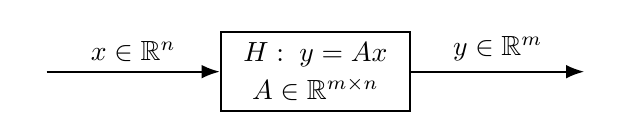
\begin{tikzpicture}[node distance=2.2cm]
  \node (in) {};
  \node[block, right=of in] (A) {$H:\; y=Ax$ \\[2pt] $A\in\mathbb{R}^{m\times n}$};
  \node[right=of A] (out) {};
  \draw[conn] (in) -- node[above] {$x\in\mathbb{R}^n$} (A);
  \draw[conn] (A) -- node[above] {$y\in\mathbb{R}^m$} (out);
\end{tikzpicture}
\caption{A system as a linear map implemented by matrix multiplication.}
\end{figure}

\subsection{Example: An amplifier as a system}
An amplifier is a system that takes in an input signal $x(t)$ and produces an output signal $y(t)$ by amplifying the input signal by a constant factor $\alpha \in \mathbb{R}$. The system can be represented as:
\[
    H: x(t) \mapsto y(t) = \alpha x(t)
\]
where $H$ is the system that amplifies the input signal by the factor $\alpha$. We can draw a block diagram of the system as follows:
\begin{figure}[h]
\centering
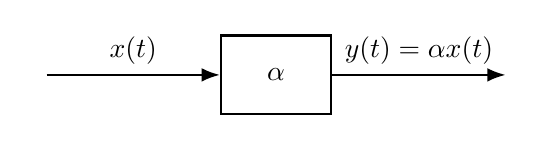
\begin{tikzpicture}[node distance=2.2cm]
  \node (xin) {};
  \node[gain, right=of xin] (G) {$\alpha$};
  \node[right=of G] (yout) {};
  \draw[conn] (xin) -- node[above] {$x(t)$} (G);
  \draw[conn] (G) -- node[above] {$y(t)=\alpha x(t)$} (yout);
\end{tikzpicture}
\caption{Amplifier system: multiply the input by a real gain \(\alpha\).}
\end{figure}
\subsection{Example: A differential equation as a system}
A system can also be represented by a differential equation that relates the input signal $x(t)$ and the output signal $y(t)$. For example, consider the following first-order linear differential equation:
\[
    \frac{dy(t)}{dt} + ay(t) = bx(t)
\]
where $a$ and $b$ are constants. This equation describes a system that takes in the input signal $x(t)$ and produces the output signal $y(t)$ by solving the differential equation.
In this case, the block diagram of the system can be represented as:
% put once in preamble
\usetikzlibrary{arrows.meta,positioning,calc}
\tikzset{
  >={Latex[length=2mm]},
  block/.style={draw, thick, rectangle, minimum height=10mm, minimum width=22mm, align=center},
  gain/.style={block, minimum width=10mm},
  sum/.style={draw, thick, circle, inner sep=0pt, minimum size=6mm},
  conn/.style={-Latex, thick},
}

% figure
\begin{figure}[h]
\centering
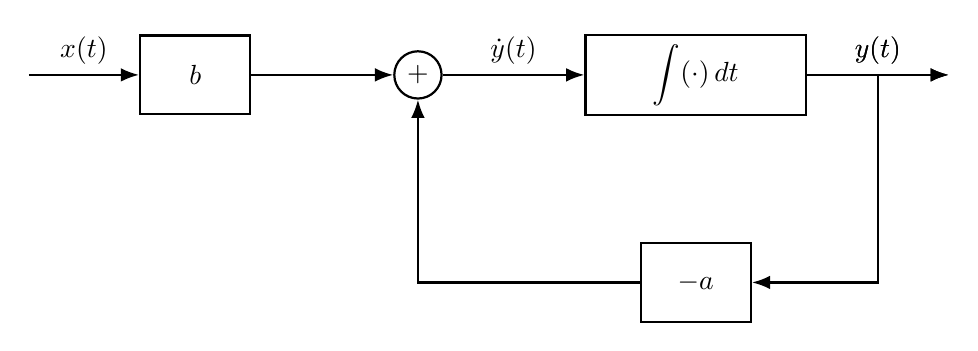
\begin{tikzpicture}[node distance=14mm]
  % nodes
  \node[coordinate] (xin) {};
  \node[gain, right=of xin] (Gb) {$b$};
  \node[sum, right=18mm of Gb] (sum) {$+$};
  \node[block, right=18mm of sum, minimum width=28mm] (Int) {$\displaystyle \int(\cdot)\,dt$};
  \node[coordinate, right=18mm of Int] (yout) {};
  \node[gain, below=16mm of Int] (Ga) {$-a$};

  % connections
  \draw[conn] (xin) -- node[above] {$x(t)$} (Gb.west);
  \draw[conn] (Gb.east) -- (sum.west);
  \draw[conn] (sum.east) -- node[above] {$\dot y(t)$} (Int.west);
  \draw[conn] (Int.east) -- node[above] {$y(t)$} (yout);

  % feedback path (tap from integrator output)
  % % get feedback path from middle of the yout arrow
\draw[conn] (Int.east) -- node[above] {$y(t)$} coordinate[pos=0.5] (ytap) (yout);
\draw[conn] (ytap) |- (Ga.east);
  \draw[conn] (Ga.west) -| (sum.south);
  % optional plus labels at summer inputs (the - sign is in the feedback gain)
  % \node at ($(sum)+(-0.35,0.28)$) {\scriptsize $+$};
  % \node at ($(sum)+(-0.35,-0.30)$) {\scriptsize $+$};
\end{tikzpicture}
\caption{Realization of \(\dot y(t)+a\,y(t)=b\,x(t)\).}
\end{figure}

\subsection{Example: A frequency modulation system}
A frequency modulation (FM) system is a system that takes in an input signal $x(t)$ and produces an output signal $y(t)$ by modulating the frequency of a carrier signal. 

\begin{popquiz}
For a purely sinusoidal audio signal $x(t) = A\cos(\omega_0 t)$, define a frequency modulator system that produces an output signal $y(t)$ that has a different frequency than the input signal. What are various ways in which you can achieve this? Can you think of a general approach to create such a system by leveraging the properties of the complex exponential signal (see previous chapter of the notes)?
\popqsplit
If you define the system as a multiplication of the input signal with $\Re\{A e^{j\omega_0 t}\}$, you will see that the output signal has a frequency that is shifted by $\omega_0$ from the input signal. 
\end{popquiz}
Consider a specific example where $x(t) = e^{j 2 \pi (10 t)}$ and we send this input through a modulator system that multiplies $e^{j 2 \pi (32 t)}$ to the input signal. The output can be obtained by computing the shift in frequency (exponents get added on multiplication). The output signal $y(t)$ for both the real and imaginary parts of the complex exponential modulator system is shown in Figure~\ref{fig:fm_sine}. 
\begin{figure}[ht]
    \centering
    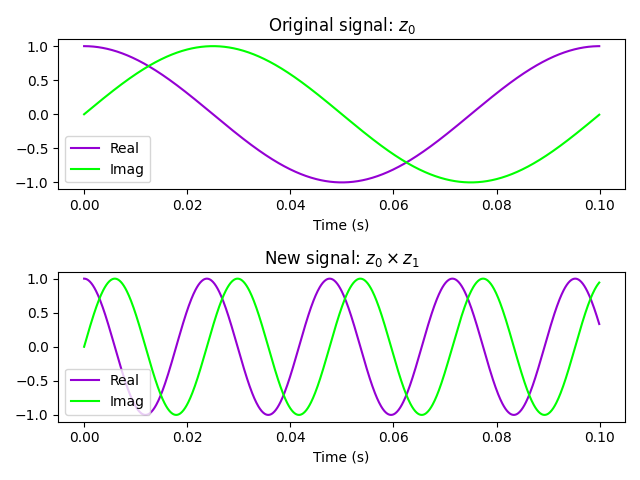
\includegraphics[width=\textwidth]{figs/fm_sine.png} 
    \caption{Frequency modulation of a sinusoidal signal using multiplication with a complex exponential.}
    \label{fig:fm_sine}
\end{figure}

An audio signal can be thought of as a combination of many sinusoidal signals with different frequencies. So, we can leverage the properties of the general complex exponential signal to define the input audio signal $x(t)$ as a sum of complex exponentials:
\[
    x(t) = \sum_{k} \Re\left(A_k e^{j\omega_k t}\right)
\]
where $A_k$ and $\omega_k$ are the amplitude and frequency of the $k$-th sinusoidal component of the audio signal. Note that for simplicity, we are just considering the cosine component. To keep it general, we can continue to work with complex numbers as it allows us to take into account both sine and cosine components (orthogonally phase shifted by $\pi/2$, which is important in representing a general signal). If we define our system as a multiplication of the input signal with $\Re\{A e^{j\omega_0 t}\}$, we will see that the output signal has a frequency that is shifted by $\omega_0$ from the input signal. The system can be represented as:
\[
    H: x(t) \mapsto y(t) = x(t) \cdot \Re\{A e^{j\omega_0 t}\}
\]
where $H$ is the system that modulates the frequency of the input signal by multiplying it with a carrier signal $\Re\{A e^{j\omega_0 t}\}$. In this case, the output $y(t)$ can be written as a sum of sinusoidal signals with frequencies shifted by $\omega_0$:
\[
    y(t) = \sum_{k} \Re\left(A_k e^{j(\omega_k + \omega_0) t}\right)
\]
For a real audio signal that you can find on course Github: \href{https://github.com/ee-ucmerced/ee102-signals-systems/blob/main/lecture\_notes/week3\_systems/guitar\_clean.wav}{guitar\_clean.wav}, we can create the simple frequency modulator using the multiplication of a complex exponential. The input and the output signals are shown in Figure~\ref{fig:fm_guitar}. You can interactively visualize and interpret the frequency of the output signal by running the virtual manipulator on frequency modulator using complex exponentials: \href{https://github.com/ee-ucmerced/ee102-signals-systems/blob/main/lecture\_notes/week3\_systems/VM\_modulation.py}{VM\_modulation.py}.
\begin{figure}[ht]
    \centering
    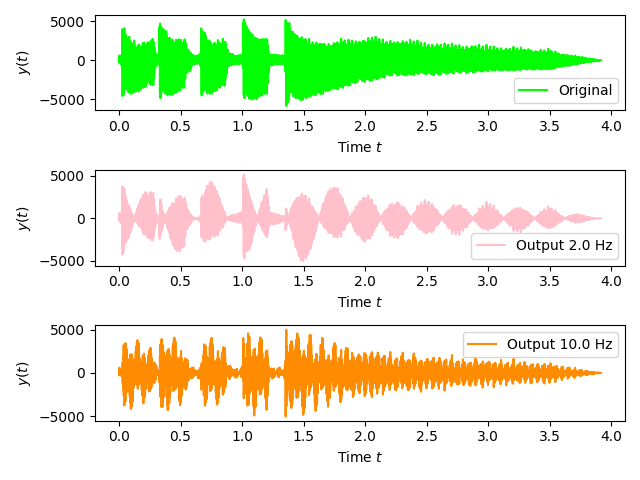
\includegraphics[width=\textwidth]{figs/fm_guitar.png} 
    \caption{Frequency modulation of a guitar audio signal using multiplication with a complex exponential.}
    \label{fig:fm_guitar}
\end{figure}
\begin{popquiz}
  By using the virtual manipulator \href{https://github.com/ee-ucmerced/ee102-signals-systems/blob/main/lecture\_notes/week3\_systems/VM\_modulation.py}{VM\_modulation.py}, test three different frequencies of the modulator system: 0.5 Hz, 5 Hz, and 20 Hz. Reflect on the expected sound for each modulation before listening to the output \texttt{guitar\_modulated.wav}. Which one of the output signals is closest to the original audio signal? How would you describe the frequency modulation effect on audio?
  \popqsplit
  The 0.5 Hz modulation is closest to the original audio signal. The frequency modulation effect on audio can be described as a shift in the frequency spectrum of the original signal, resulting in a change in the perceived pitch and timbre of the sound, which ends up sounding like a reverberation.
\end{popquiz}
\begin{popquiz}
  Can you define a noise cancellation system that takes in a noisy signal and produces an output signal that cancels the noise? Assume that the noise is a sinusoidal signal with a known frequency and amplitude. 
  \popqsplit
  See Problem 1 on Homework 3.
\end{popquiz}

\section{Properties of Systems}
Systems can have various properties that define their behavior and characteristics. Some of the most common properties of systems are:
\begin{itemize}
    \item \textbf{Linearity:} A system is linear if it satisfies the principles of superposition and homogeneity. This means that the output of the system for a linear combination of input signals is equal to the same linear combination of the outputs for each individual input signal.
    \item \textbf{Time-invariance:} A system is time-invariant if its behavior and characteristics do not change over time. This means that if the input signal is shifted in time, the output signal will also be shifted by the same amount.
    \item \textbf{Causality:} A system is causal if the output at any given time depends only on the current and past input values, and not on future input values. In other words, a causal system cannot anticipate future inputs.
    \item \textbf{Memory:} A system has memory if its output depends on past input values. A system without memory (also called memoryless) produces an output that depends only on the current input value.
    \item \textbf{Invertibility:} A system is invertible if there exists an inverse system that can recover the original input signal from the output signal. In other words, if you apply the inverse system to the output, you should get back the original input.
    \item \textbf{Stability:} A system is ``BIBO'' stable if bounded input signals produce bounded output signals. This means that if the input signal remains within a certain range, the output signal will also remain within a certain range (bounded input implies bounded output: BIBO).
\end{itemize}
\begin{popquiz}
  Can you find a positive and a negative system example of each of the properties listed above? For example, for the memory property, the ``positive'' would be a system that has memory, and the ``negative'' would be a system that is memoryless. 
  \popqsplit
  Here are some examples:
  \begin{itemize}
      \item Linearity: Positive - Amplifier system $y(t) = \alpha x(t)$; Negative - Clipping system $y(t) = \text{clip}(x(t))$ is nonlinear.
      \item Time-invariance: Positive - Delay system $y(t) = x(t - t_0)$; Negative - Time-varying gain system $y(t) = t x(t)$.
      \item Causality: Positive - Delay system $y(t) = x(t - t_0)$; Negative - Anticipatory system $y(t) = x(t + t_0)$ for $t_0 >0$.
      \item Memory: Positive - Integrator system $y(t) = \int_{-\infty}^{t} x(\tau) d\tau$; Negative - Memoryless system $y(t) = x(t)^2$ only depends on the current instant of time.
      \item Invertibility: Positive - Scaling system $y(t) = 2x(t)$; Negative - Clipping system $y(t) = \text{clip}(x(t))$ cannot be inverted as all values lead to the same clipped behavior after a certain threshold.
      \item Stability: Positive - An RC circuit with decaying voltage: $y(t) = (1 - e^{-t/\tau}) x(t)$; Negative - Unstable system (e.g., $y(t) = e^{t} x(t)$).
  \end{itemize} 
\end{popquiz}
A common type of system that we will end up studying is a causal stable LTI system. Causality is important because we will be studying time-domain signals. To ensure that signals don't blow up to $\infty$, we require stability. Finally, LTI systems, or linear time-invariant systems, will be the central class of systems we will study due to their nice properties and because many useful practical signals can be modeled as LTI systems.
\subsection{Example: LTI system response}
By using linearity and time-invariance, we can analyze the response of an LTI system to inputs and initial conditions. Consider the system with three different inputs: $x_1(t)$, $x_2(t)$, and $x_3(t)$. Define the output of the system for each of the signals as $y_1(t)$, $y_2(t)$, and $y_3(t)$ respectively. Let us assume that the system is also affected by its initial conditions $q_1(0)$ and $q_2(0)$. 

We denote $y_i^{\mathrm{ZS}}(t)$ as the zero-state output due to $x_i(t)$ with all initial conditions set to zero. Further, we denote $y_{q_1}(t)$ and $y_{q_2}(t)$ as the zero-input outputs produced by initial conditions in those two modes (with external inputs, $x_i$, set to zero).

Then, for any scalars $\alpha_1,\dots,\alpha_5$,
\[
x(t)=\alpha_1 x_1(t)+\alpha_2 x_2(t)+\alpha_3 x_3(t),\quad
q(0)=\alpha_4\,q_1(0)+\alpha_5\,q_2(0)
\]
\[
~\Longrightarrow~
y(t)=\alpha_1 y_1^{\mathrm{ZS}}(t)+\alpha_2 y_2^{\mathrm{ZS}}(t)+\alpha_3 y_3^{\mathrm{ZS}}(t)
      +\alpha_4 y_{q_1}(t)+\alpha_5 y_{q_2}(t).
\]
Note that it is essential that $y_i^{\mathrm{ZS}}$ are computed with zero initial conditions otherwise the initial contributions would be double-counted. Likewise, $y_{q_1},y_{q_2}$ are computed with zero external input.

Further, if one of the inputs is shifted in time, say $x_3(t-t_0)$, then by the time-invariance property of the system, the output is also shifted by the same amount:
\[
x(t)=\alpha_1 x_1(t)+\alpha_2 x_2(t)+\alpha_3 x_3(t-t_0),\quad
q(0)=\alpha_4\,q_1(0)+\alpha_5\,q_2(0)
\]
\[
~\Longrightarrow~
y(t)=\alpha_1 y_1^{\mathrm{ZS}}(t)+\alpha_2 y_2^{\mathrm{ZS}}(t)+\alpha_3 y_3^{\mathrm{ZS}}(t-t_0)
      +\alpha_4 y_{q_1}(t)+\alpha_5 y_{q_2}(t).
\]
\end{document}